\documentclass{standalone}
\usepackage{tikz}
\usetikzlibrary{patterns}
\usetikzlibrary{positioning}
\usetikzlibrary{patterns, positioning}
\usetikzlibrary{shapes.misc}
\usepackage[outline]{contour}
\contourlength{1.5pt} 
\usepackage[sfdefault]{ClearSans}

\begin{document}
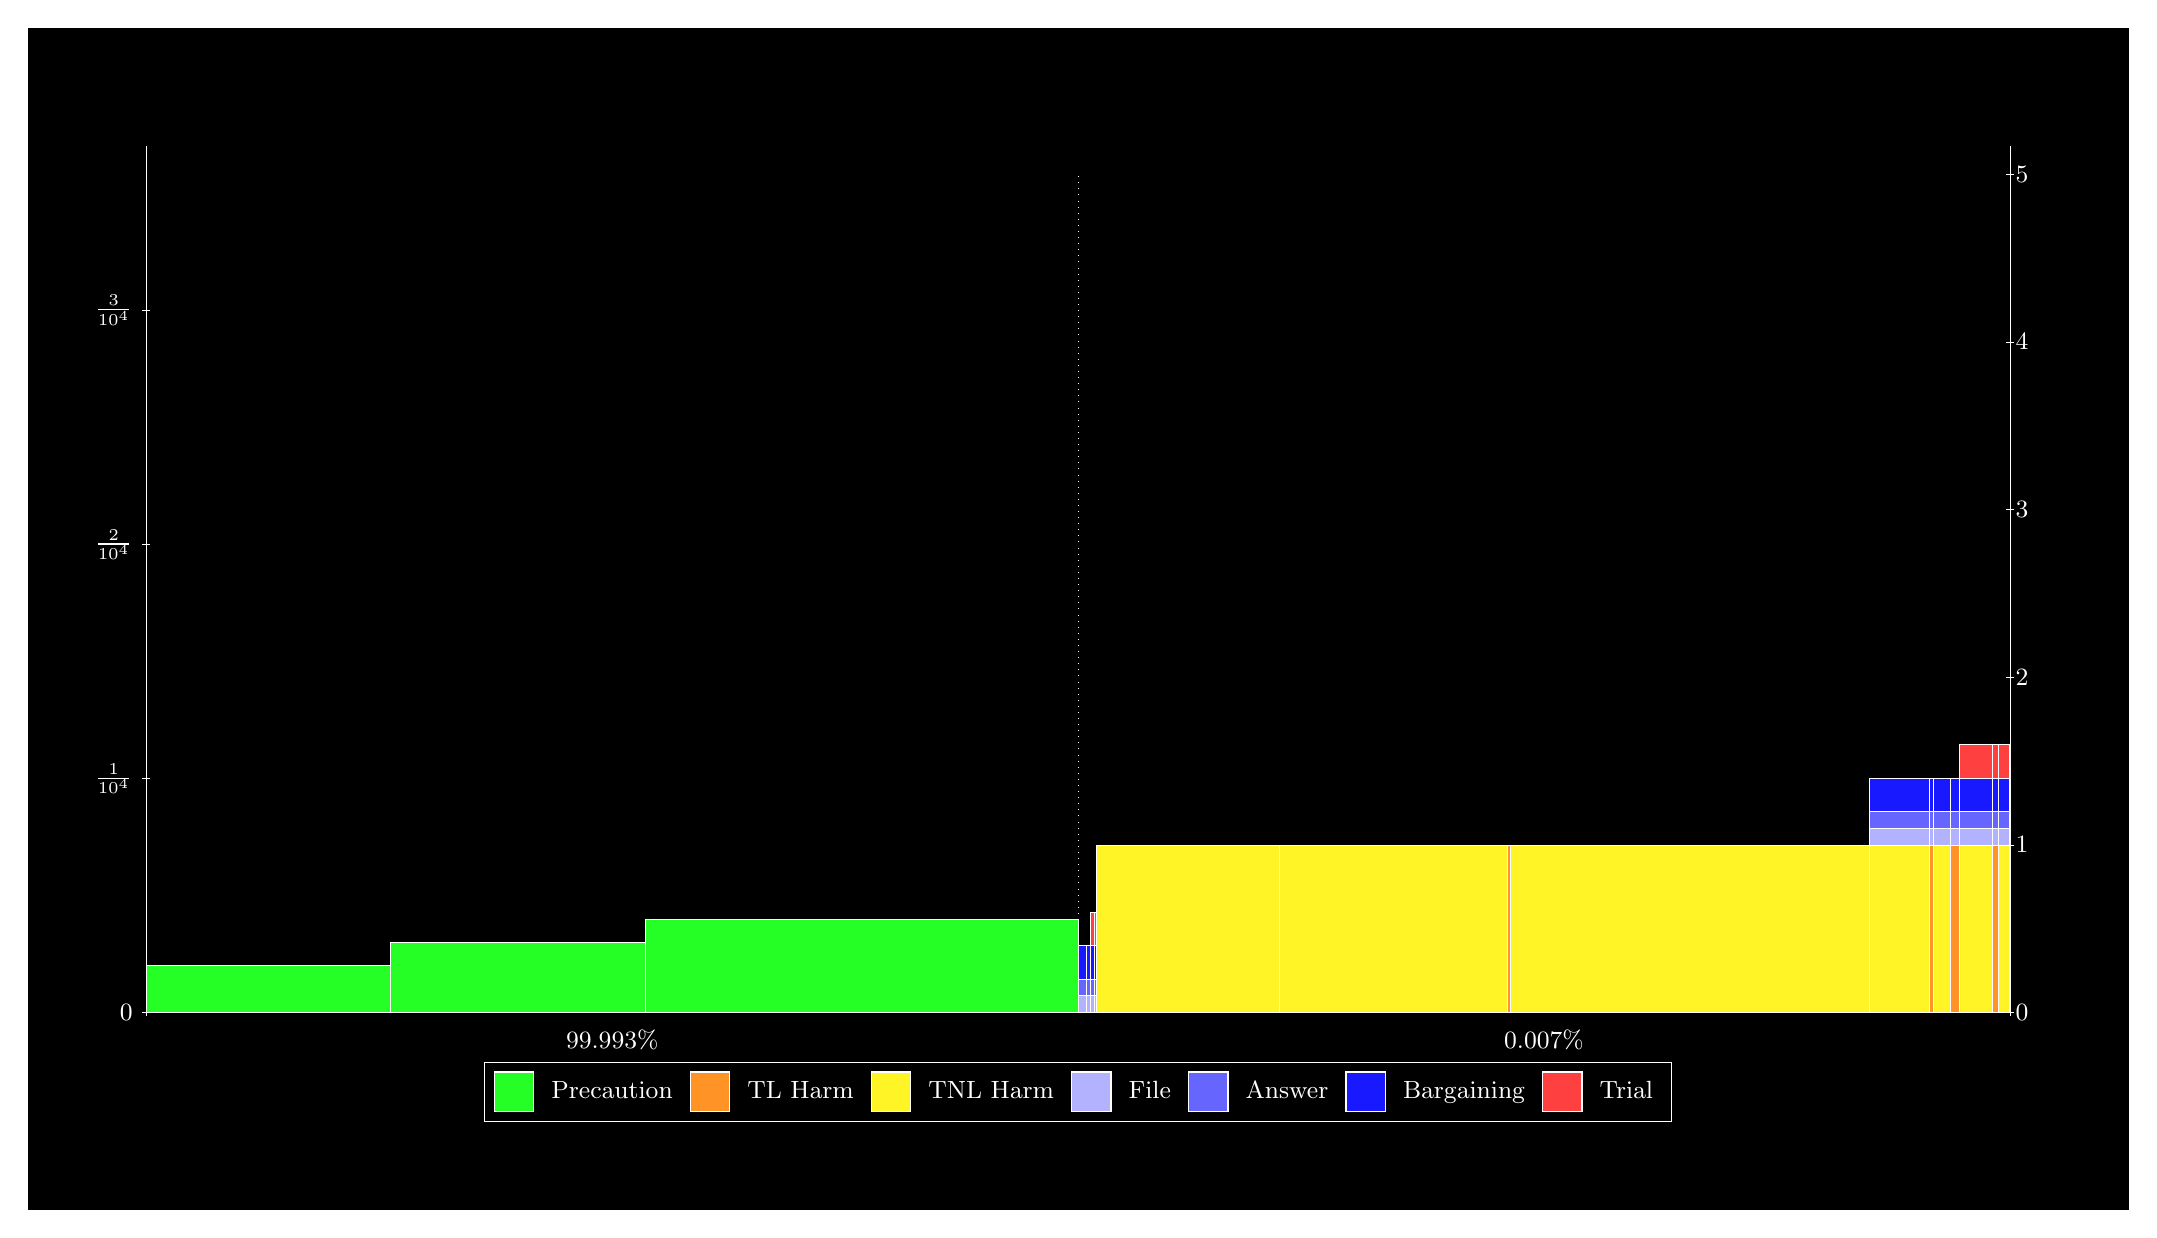
\begin{tikzpicture}
\draw[fill=black] (0,0) rectangle (26.667,15);
\draw[fill=green!85,draw=white,very thin] (1.5,2.5) rectangle (4.5971,3.0946);
\draw[fill=green!85,draw=white,very thin] (4.5971,2.5) rectangle (7.8387,3.3918);
\draw[fill=green!85,draw=white,very thin] (7.8387,2.5) rectangle (13.333,3.6891);
\draw[fill=green!85,draw=white,very thin] (13.333,2.5) rectangle (13.434,2.5);
\draw[fill=blue!30,draw=white,very thin] (13.333,2.5) rectangle (13.434,2.7129);
\draw[fill=blue!60,draw=white,very thin] (13.333,2.7129) rectangle (13.434,2.9258);
\draw[fill=blue!90,draw=white,very thin] (13.333,2.9258) rectangle (13.434,3.3516);
\draw[fill=green!85,draw=white,very thin] (13.434,2.5) rectangle (13.484,2.5001);
\draw[fill=blue!30,draw=white,very thin] (13.434,2.5001) rectangle (13.484,2.713);
\draw[fill=blue!60,draw=white,very thin] (13.434,2.713) rectangle (13.484,2.9259);
\draw[fill=blue!90,draw=white,very thin] (13.434,2.9259) rectangle (13.484,3.3517);
\draw[fill=green!85,draw=white,very thin] (13.484,2.5) rectangle (13.545,2.5);
\draw[fill=blue!30,draw=white,very thin] (13.484,2.5) rectangle (13.545,2.7129);
\draw[fill=blue!60,draw=white,very thin] (13.484,2.7129) rectangle (13.545,2.9258);
\draw[fill=blue!90,draw=white,very thin] (13.484,2.9258) rectangle (13.545,3.3516);
\draw[fill=red!75,draw=white,very thin] (13.484,3.3516) rectangle (13.545,3.7774);
\draw[fill=green!85,draw=white,very thin] (13.545,2.5) rectangle (13.566,2.5001);
\draw[fill=blue!30,draw=white,very thin] (13.545,2.5001) rectangle (13.566,2.713);
\draw[fill=blue!60,draw=white,very thin] (13.545,2.713) rectangle (13.566,2.9259);
\draw[fill=blue!90,draw=white,very thin] (13.545,2.9259) rectangle (13.566,3.3517);
\draw[fill=red!75,draw=white,very thin] (13.545,3.3517) rectangle (13.566,3.7774);
\draw[fill=green!85,draw=white,very thin] (13.566,2.5) rectangle (15.886,2.5);
\draw[fill=yellow!85,draw=white,very thin] (13.566,2.5) rectangle (15.886,4.629);
\draw[fill=green!85,draw=white,very thin] (15.886,2.5) rectangle (18.786,2.5001);
\draw[fill=yellow!85,draw=white,very thin] (15.886,2.5001) rectangle (18.786,4.629);
\draw[fill=green!85,draw=white,very thin] (18.786,2.5) rectangle (18.826,2.5001);
\draw[fill=orange!85,draw=white,very thin] (18.786,2.5001) rectangle (18.826,4.629);
\draw[fill=green!85,draw=white,very thin] (18.826,2.5) rectangle (23.385,2.5001);
\draw[fill=yellow!85,draw=white,very thin] (18.826,2.5001) rectangle (23.385,4.6291);
\draw[fill=green!85,draw=white,very thin] (23.385,2.5) rectangle (24.137,2.5);
\draw[fill=yellow!85,draw=white,very thin] (23.385,2.5) rectangle (24.137,4.629);
\draw[fill=blue!30,draw=white,very thin] (23.385,4.629) rectangle (24.137,4.8419);
\draw[fill=blue!60,draw=white,very thin] (23.385,4.8419) rectangle (24.137,5.0548);
\draw[fill=blue!90,draw=white,very thin] (23.385,5.0548) rectangle (24.137,5.4806);
\draw[fill=green!85,draw=white,very thin] (24.137,2.5) rectangle (24.196,2.5);
\draw[fill=orange!85,draw=white,very thin] (24.137,2.5) rectangle (24.196,4.629);
\draw[fill=blue!30,draw=white,very thin] (24.137,4.629) rectangle (24.196,4.8419);
\draw[fill=blue!60,draw=white,very thin] (24.137,4.8419) rectangle (24.196,5.0548);
\draw[fill=blue!90,draw=white,very thin] (24.137,5.0548) rectangle (24.196,5.4806);
\draw[fill=green!85,draw=white,very thin] (24.196,2.5) rectangle (24.406,2.5001);
\draw[fill=yellow!85,draw=white,very thin] (24.196,2.5001) rectangle (24.406,4.629);
\draw[fill=blue!30,draw=white,very thin] (24.196,4.629) rectangle (24.406,4.8419);
\draw[fill=blue!60,draw=white,very thin] (24.196,4.8419) rectangle (24.406,5.0548);
\draw[fill=blue!90,draw=white,very thin] (24.196,5.0548) rectangle (24.406,5.4806);
\draw[fill=green!85,draw=white,very thin] (24.406,2.5) rectangle (24.518,2.5001);
\draw[fill=orange!85,draw=white,very thin] (24.406,2.5001) rectangle (24.518,4.629);
\draw[fill=blue!30,draw=white,very thin] (24.406,4.629) rectangle (24.518,4.8419);
\draw[fill=blue!60,draw=white,very thin] (24.406,4.8419) rectangle (24.518,5.0548);
\draw[fill=blue!90,draw=white,very thin] (24.406,5.0548) rectangle (24.518,5.4806);
\draw[fill=green!85,draw=white,very thin] (24.518,2.5) rectangle (24.949,2.5);
\draw[fill=yellow!85,draw=white,very thin] (24.518,2.5) rectangle (24.949,4.629);
\draw[fill=blue!30,draw=white,very thin] (24.518,4.629) rectangle (24.949,4.8419);
\draw[fill=blue!60,draw=white,very thin] (24.518,4.8419) rectangle (24.949,5.0548);
\draw[fill=blue!90,draw=white,very thin] (24.518,5.0548) rectangle (24.949,5.4806);
\draw[fill=red!75,draw=white,very thin] (24.518,5.4806) rectangle (24.949,5.9064);
\draw[fill=green!85,draw=white,very thin] (24.949,2.5) rectangle (25.016,2.5);
\draw[fill=orange!85,draw=white,very thin] (24.949,2.5) rectangle (25.016,4.629);
\draw[fill=blue!30,draw=white,very thin] (24.949,4.629) rectangle (25.016,4.8419);
\draw[fill=blue!60,draw=white,very thin] (24.949,4.8419) rectangle (25.016,5.0548);
\draw[fill=blue!90,draw=white,very thin] (24.949,5.0548) rectangle (25.016,5.4806);
\draw[fill=red!75,draw=white,very thin] (24.949,5.4806) rectangle (25.016,5.9064);
\draw[fill=green!85,draw=white,very thin] (25.016,2.5) rectangle (25.163,2.5001);
\draw[fill=yellow!85,draw=white,very thin] (25.016,2.5001) rectangle (25.163,4.629);
\draw[fill=blue!30,draw=white,very thin] (25.016,4.629) rectangle (25.163,4.8419);
\draw[fill=blue!60,draw=white,very thin] (25.016,4.8419) rectangle (25.163,5.0548);
\draw[fill=blue!90,draw=white,very thin] (25.016,5.0548) rectangle (25.163,5.4806);
\draw[fill=red!75,draw=white,very thin] (25.016,5.4806) rectangle (25.163,5.9064);
\draw[fill=green!85,draw=white,very thin] (25.163,2.5) rectangle (25.167,2.5001);
\draw[fill=orange!85,draw=white,very thin] (25.163,2.5001) rectangle (25.167,4.629);
\draw[fill=blue!30,draw=white,very thin] (25.163,4.629) rectangle (25.167,4.8419);
\draw[fill=blue!60,draw=white,very thin] (25.163,4.8419) rectangle (25.167,5.0548);
\draw[fill=blue!90,draw=white,very thin] (25.163,5.0548) rectangle (25.167,5.4806);
\draw[fill=red!75,draw=white,very thin] (25.163,5.4806) rectangle (25.167,5.9064);
\draw[white,very thin] (1.5,2.5) -- (1.5,13.5);
\draw[white,very thin] (1.45,2.5) -- (1.55,2.5);
\node[font=\small,text=white, anchor=east] at (1.45, 2.5) {0};
\draw[white,very thin] (1.45,5.4728) -- (1.55,5.4728);
\node[font=\small,text=white, anchor=east] at (1.45, 5.4728) {$\frac{1}{10^{4}}$};
\draw[white,very thin] (1.45,8.4455) -- (1.55,8.4455);
\node[font=\small,text=white, anchor=east] at (1.45, 8.4455) {$\frac{2}{10^{4}}$};
\draw[white,very thin] (1.45,11.418) -- (1.55,11.418);
\node[font=\small,text=white, anchor=east] at (1.45, 11.418) {$\frac{3}{10^{4}}$};

\draw[white,dotted,very thin] (13.333,2.83) -- (13.333,13.17);
\draw[white,very thin] (25.167,2.5) -- (25.167,13.5);
\draw[white,very thin] (25.117,2.5) -- (25.217,2.5);
\node[font=\small,text=white, anchor=west] at (25.117, 2.5) {0};
\draw[white,very thin] (25.117,4.629) -- (25.217,4.629);
\node[font=\small,text=white, anchor=west] at (25.117, 4.629) {1};
\draw[white,very thin] (25.117,6.7579) -- (25.217,6.7579);
\node[font=\small,text=white, anchor=west] at (25.117, 6.7579) {2};
\draw[white,very thin] (25.117,8.8869) -- (25.217,8.8869);
\node[font=\small,text=white, anchor=west] at (25.117, 8.8869) {3};
\draw[white,very thin] (25.117,11.016) -- (25.217,11.016);
\node[font=\small,text=white, anchor=west] at (25.117, 11.016) {4};
\draw[white,very thin] (25.117,13.145) -- (25.217,13.145);
\node[font=\small,text=white, anchor=west] at (25.117, 13.145) {5};

\draw[white,very thin] (1.5,2.5) -- (25.167,2.5);
\draw[white,very thin] (1.5,2.45) -- (1.5,2.55);
\node[font=\small,text=white, anchor=north] at (1.5, 2.45) {};
\draw[white,very thin] (25.167,2.45) -- (25.167,2.55);
\node[font=\small,text=white, anchor=north] at (25.167, 2.45) {};

\node[font=\small,text=white,anchor=south] at (7.4167, 1.9) {99.993\%};
\node[font=\small,text=white,anchor=south] at (19.25, 1.9) {0.007\%};
\draw (13.3333,2.5) node (B) {};
\begin{scope}[align=center]
\matrix[scale=0.5,draw=white,below=0.5cm of B,nodes={draw},column sep=0.1cm]{
\node[rectangle,draw,minimum width=0.5cm,minimum height=0.5cm,fill=green!85]{}; & \node[draw=none,font=\small,text=white]{Precaution}; &
\node[rectangle,draw,minimum width=0.5cm,minimum height=0.5cm,fill=orange!85]{}; & \node[draw=none,font=\small,text=white]{TL Harm}; &
\node[rectangle,draw,minimum width=0.5cm,minimum height=0.5cm,fill=yellow!85]{}; & \node[draw=none,font=\small,text=white]{TNL Harm}; &
\node[rectangle,draw,minimum width=0.5cm,minimum height=0.5cm,fill=blue!30]{}; & \node[draw=none,font=\small,text=white]{File}; &
\node[rectangle,draw,minimum width=0.5cm,minimum height=0.5cm,fill=blue!60]{}; & \node[draw=none,font=\small,text=white]{Answer}; &
\node[rectangle,draw,minimum width=0.5cm,minimum height=0.5cm,fill=blue!90]{}; & \node[draw=none,font=\small,text=white]{Bargaining}; &
\node[rectangle,draw,minimum width=0.5cm,minimum height=0.5cm,fill=red!75]{}; & \node[draw=none,font=\small,text=white]{Trial}; \\\\
};\end{scope}

\end{tikzpicture}
\end{document}